\documentclass[manuscript,screen,review]{acmart}

\usepackage{booktabs}
\usepackage{tabularx}
\usepackage{array}
\usepackage{multirow}
\usepackage{graphicx}
\newcolumntype{Y}{>{\raggedright\arraybackslash}X}

% TODO before formal submission:
% 1. If the target venue uses double-blind review, add "anonymous" to the
%    documentclass options.
% 2. Replace all author, affiliation, conference, copyright, DOI, ISBN, and
%    CCS placeholders with venue-confirmed metadata.
% 3. Confirm whether the current figures and references satisfy the target venue.

\setcopyright{none}
\settopmatter{printacmref=true, printccs=true, printfolios=true}

\acmConference[Conference Placeholder '26]{Proceedings Placeholder}{Month DD--DD, 2026}{City, Country}
\acmBooktitle{Proceedings Placeholder}
\acmYear{2026}
\copyrightyear{2026}
\acmDOI{10.1145/0000000.0000000}
\acmISBN{978-1-4503-0000-0/26/06}

\newcommand{\msat}{MSAT}
\newcommand{\px}{PU-XMSAT}
\newcommand{\cmmadr}{CMM--ADR}
\graphicspath{{figures/}}

\title[PU-XMSAT for CMM Adverse Reaction Prediction]{PU-XMSAT: Positive-Unlabeled Learning and Mechanism-Guided Interpretation for Chinese Materia Medica Adverse Reaction Prediction}

\author{First Author}
\affiliation{%
  \institution{Institution Placeholder}
  \city{City}
  \country{Country}
}
\email{first.author@example.com}

\author{Second Author}
\affiliation{%
  \institution{Institution Placeholder}
  \city{City}
  \country{Country}
}
\email{second.author@example.com}

\author{Corresponding Author}
\authornote{Corresponding author.}
\affiliation{%
  \institution{Institution Placeholder}
  \city{City}
  \country{Country}
}
\email{corresponding.author@example.com}

\renewcommand{\shortauthors}{First Author et al.}

\begin{abstract}
Predicting adverse reactions associated with Chinese materia medica is challenging because observed adverse-reaction databases are incomplete: an unreported herb--adverse drug reaction pair is not necessarily a true negative. We first reproduced the \msat{} protocol as the experimental anchor and then developed \px{}, a positive-unlabeled extension that separates observed positive pairs, reliable negative pairs, and down-weighted unlabeled pairs. Under the same ten-fold protocol as the reproduced \msat{} baseline, the full-positive hybrid \px{} setting achieved seed-robust improvements in AUC, F1, and MCC, with a stable positive but smaller AUPRC trend. Across two seeds, hybrid \px{} reached AUC around 0.9804, AUPRC around 0.9780, F1 around 0.9348--0.9351, and MCC around 0.8683--0.8684. To support cautious interpretation, we further added a mechanism-oriented analysis layer that extracts key subgraphs and quantifies local node- and path-level perturbation sensitivity for selected cases. The current evidence supports \px{} as a conservative incomplete-label mitigation and mechanism-prioritization framework, while case-level external validation and causal effect estimation remain outside the supported claim boundary.
\end{abstract}

% TODO: replace these with verified ACM CCS concepts from https://dl.acm.org/ccs
\ccsdesc[500]{Computing methodologies~Machine learning}
\ccsdesc[300]{Applied computing~Health informatics}
\ccsdesc[300]{Information systems~Data mining}

\keywords{positive-unlabeled learning, Chinese materia medica, adverse reaction prediction, graph neural networks, mechanism interpretation, pharmacovigilance}

\begin{document}

\maketitle

\section{Introduction}

Chinese materia medica (CMM) is widely used in clinical and community settings, but adverse reaction prediction remains difficult because safety evidence is fragmented across heterogeneous databases, case reports, molecular resources, and expert knowledge. This fragmentation is especially important for traditional Chinese medicine safety, where adverse reactions can involve multi-component preparations, variable product quality, co-medication, and incomplete reporting \cite{chan2015overview,wu2010recommendations}. Graph-based prediction methods have therefore become attractive for CMM adverse drug reaction (ADR) discovery because they can connect herbs, compounds, targets, biological mechanisms, and adverse reaction labels in a shared representation space.

The \msat{} model provides a useful foundation for this task by combining multi-source graph information for CMM--ADR association prediction. However, reproducing and extending such a model exposes an important supervision issue: in adverse-reaction data, unobserved pairs are not guaranteed to be true negatives. Spontaneous reporting systems are useful for signal generation, but under-reporting and reporting bias are well-known limitations \cite{hazell2006underreporting,bate2009quantitative}. A herb--ADR pair may be absent because it has not been reported, because the exposed population is small, because reporting is biased, or because relevant evidence is difficult to curate. Treating all unobserved pairs as negative samples can therefore introduce incomplete-label noise.

The research value of this study is therefore methodological as well as practical. Methodologically, it asks whether a high-performing graph model can be improved without changing its architecture, simply by correcting a supervision assumption that is especially fragile in pharmacovigilance. Practically, it turns the reproduced \msat{} pipeline into a more cautious risk-prioritization workflow: predictions are evaluated under the same folds, interpreted through mechanism subgraphs, and bounded by external-evidence and causal-bias checks. This makes the work useful not only as a performance extension, but also as a reproducible template for handling incomplete safety labels in CMM pharmacovigilance.

The proposed extension is positioned between reporting-based signal detection and mechanism-guided graph prediction. Disproportionality and other spontaneous-reporting analyses identify statistical reporting signals from observed reports \cite{bate2009quantitative,harpaz2012novel}. \px{} instead studies how to train a graph predictor when many candidate CMM--ADR pairs are simply unlabeled. This distinction matters for research value: the method does not replace clinical review, but it makes the negative-label assumption explicit and testable under a reproduced benchmark.

This paper studies a targeted extension of the reproduced \msat{} protocol. We propose \px{}, a positive-unlabeled learning variant that preserves the reproduced \msat{} architecture and cross-validation protocol while changing the construction and weighting of supervision pairs. Observed CMM--ADR associations are retained as positive pairs. A subset of unobserved pairs is selected as reliable negatives using a mechanism-aware candidate score, and the remaining unobserved pairs are treated as unlabeled examples with reduced training weight.

Our goal is intentionally conservative. We do not claim that \px{} proves causal effects of CMM exposure on ADR risk, nor do we claim that all auxiliary evidence tables in the original \msat{} paper have been fully reproduced. Instead, we ask whether incomplete-label treatment can improve the reproduced main prediction protocol and whether the resulting model can be paired with a transparent mechanism-prioritization workflow.

The main contributions are:
\begin{itemize}
  \item We reproduce the \msat{} experimental protocol as a baseline anchor and identify the incomplete-label limitation in treating all unobserved CMM--ADR pairs as negative samples.
  \item We implement \px{}, a positive-unlabeled extension that separates observed positives, reliable negatives, and down-weighted unlabeled pairs under the reproduced graph protocol.
  \item We show that full-positive hybrid \px{} gives seed-robust improvements over the reproduced \msat{} baseline on AUC, F1, and MCC, with a stable positive AUPRC trend.
  \item We add a bounded mechanism-interpretation layer with key subgraphs, local node and path perturbations, and aggregate ranks for case triage.
\end{itemize}

\subsection{Research Questions and Evidence Design}

To make the evaluation auditable, we organize the study around four research questions (Table~\ref{tab:rq-evidence}) and summarize the full study pipeline in Figure~\ref{fig:method-overview}. This structure separates three issues that are often conflated in pharmacovigilance prediction papers: whether the main predictive protocol improves, whether the improvement is robust to reasonable training choices, and whether the case-level interpretation is strong enough to support biological or clinical claims. In this manuscript, the strongest claim is attached to the first two questions, while the interpretation and evidence questions are used to define a conservative boundary for future review.

\begin{table*}[t]
\caption{Research questions, evidence, and claim boundaries for PU-XMSAT.}
\label{tab:rq-evidence}
\small
\begin{tabularx}{\textwidth}{p{0.08\textwidth} Y Y Y}
\toprule
ID & Question & Evidence reported in this manuscript & Claim boundary \\
\midrule
RQ1 & Does PU treatment of unobserved CMM--ADR pairs improve the reproduced MSAT main protocol? & Ten-fold comparison against the reproduced MSAT anchor using the same official folds; paired fold-level tests for AUC, AUPRC, F1, and MCC. & Supports protocol-level improvement, not universal superiority across all graph constructions or datasets. \\
RQ2 & Is the strongest PU-XMSAT setting stable rather than a single-seed artifact? & Hybrid full-positive runs under seeds 2026 and 1337, plus focused unlabeled-weight sensitivity around the default setting. & Supports local robustness around the tested setting; it does not exhaust all stochastic or hyperparameter variation. \\
RQ3 & Can the model output be connected to mechanism-level entities and paths? & Key subgraph extraction, local node/path perturbation sensitivity, and aggregate sensitivity ranking for selected mechanism-supported cases. & Supports mechanism prioritization; perturbation drops are not SHAP values, causal effects, or confirmed biological mechanisms. \\
RQ4 & Can case predictions be promoted to externally validated adverse-reaction evidence? & Evidence grading and manual review of available literature/database support for candidate cases. & Current cases remain screening candidates; no row is upgraded to confirmed external validation. \\
\bottomrule
\end{tabularx}
\end{table*}

\begin{figure*}[t]
  \centering
  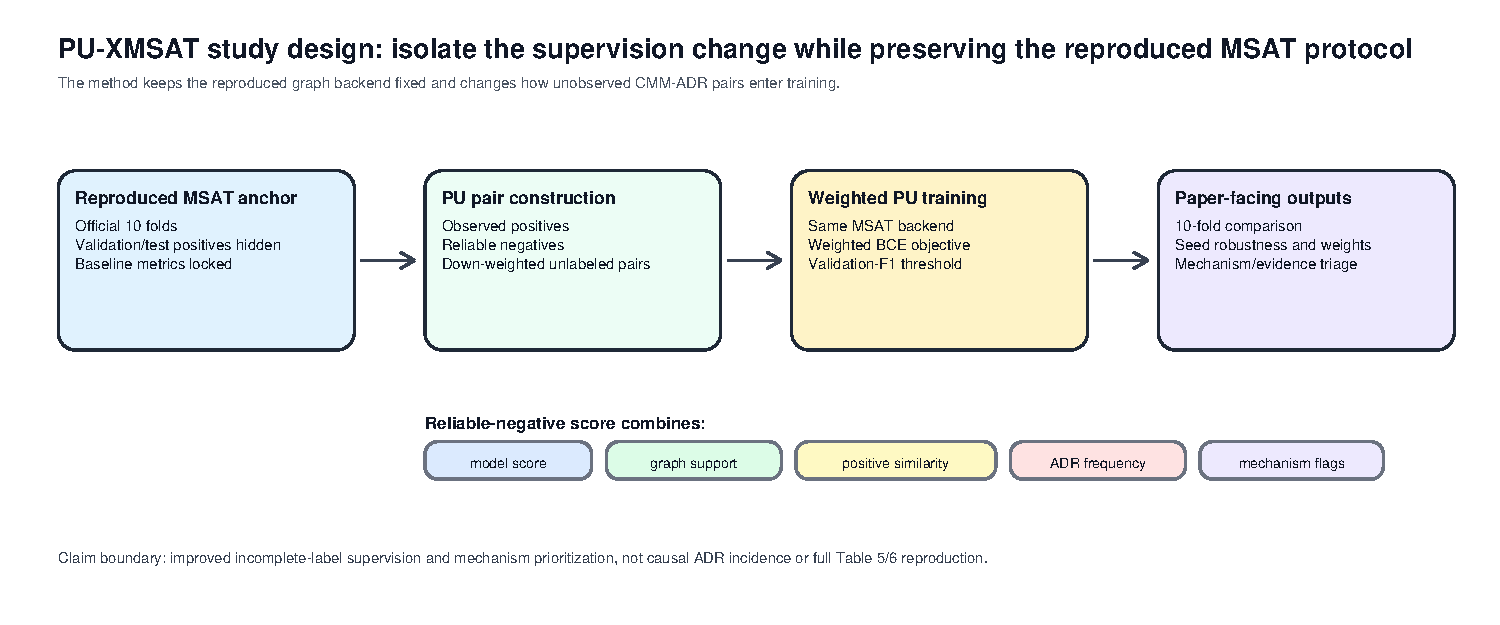
\includegraphics[width=\textwidth]{method_overview.pdf}
  \caption{Overview of the PU-XMSAT study design. The extension keeps the reproduced MSAT graph backend and fold protocol fixed, then changes the supervision construction for unobserved CMM--ADR pairs by separating reliable negatives and down-weighted unlabeled examples.}
  \Description{A left-to-right pipeline showing reproduced MSAT anchor, PU pair construction, weighted PU training, and paper-facing outputs. A second row lists the components of the reliable-negative score.}
  \label{fig:method-overview}
\end{figure*}

\section{Related Work}

\subsection{CMM Adverse Reaction Prediction}

Computational CMM safety prediction aims to prioritize potential adverse reactions before strong clinical evidence is available. Spontaneous reporting systems such as FAERS support post-marketing safety surveillance at scale, but they are noisy and affected by under-reporting, reporting bias, duplicate reports, co-medication, and incomplete exposure denominators \cite{fda_faers,hazell2006underreporting,harpaz2012novel}. Traditional Chinese medicine pharmacovigilance adds further reporting and classification challenges because herb products, preparations, and combined use patterns can be difficult to standardize \cite{chan2015overview,wu2010recommendations}. TCM-specific signal-detection studies have therefore argued for data-classification strategies that respect the structure of TCM reports rather than treating them as ordinary drug reports \cite{wei2018tcm_signal}. Existing computational approaches often use heterogeneous resources, including herb--compound relationships, compound--target interactions, disease or pathway annotations, and known adverse reaction records. The \msat{} framework is representative of this graph-based direction and serves as the baseline anchor in this study \cite{msat_original}. Because our focus is reproducibility and incomplete-label extension, we keep the original model family fixed and evaluate whether changing the supervision assumption improves the reproduced protocol.

\subsection{Heterogeneous Graph Learning for Drug Safety}

Drug-safety prediction naturally forms a heterogeneous graph problem: drugs, herbs, targets, proteins, phenotypes, and adverse events are linked by typed relations. Prior graph-learning work has modeled multi-relational drug safety settings such as polypharmacy side-effect prediction \cite{zitnik2018modeling}. More general heterogeneous or relational graph neural networks also provide mechanisms for propagating evidence across typed edges \cite{schlichtkrull2018modeling,hu2020heterogeneous}. \px{} follows this relational perspective but uses it for a narrower reproducibility question: given a fixed reproduced \msat{} graph backend, does a more cautious treatment of missing CMM--ADR labels improve the main prediction protocol?

\subsection{Positive-Unlabeled Learning}

Positive-unlabeled (PU) learning addresses binary classification settings in which only positive and unlabeled examples are observed \cite{elkan2008learning,bekker2020learning,kiryo2017positive}. This formulation is well aligned with adverse-reaction discovery: the absence of a known association does not imply the absence of risk. In \px{}, we use PU learning pragmatically. Observed CMM--ADR associations are positives, selected unobserved pairs are reliable negatives, and the remaining unobserved pairs are optimized with reduced sample weight. The purpose is not to solve every source of pharmacovigilance bias, but to remove one avoidable source of supervision noise from the reproduced graph-learning protocol.

\subsection{Mechanism Interpretation and Claim Boundaries}

Interpretability is important in pharmacovigilance because a prediction score alone is rarely sufficient for biological or clinical review. Feature attribution methods such as SHAP quantify predictive contribution under specific assumptions \cite{lundberg2017unified}, while causal frameworks emphasize the distinction between association, intervention, and confounding \cite{pearl2009causality}. Our current interpretation layer is more limited: it extracts mechanism subgraphs and measures local perturbation sensitivity by masking node features or path-level feature sets. These scores are useful for triage, but they are not SHAP values, causal estimates, or direct biological validation.

\section{Materials and Methods}

\subsection{Reproduction Anchor}

We used the reproduced \msat{} protocol as the baseline anchor. The reproduction follows the same ten official folds and uses the protocol version in which validation and test positive CMM--ADR supervision edges are hidden from the training graph. This edge-hiding step is important because validation or test positive supervision edges should not be visible during training-time message passing.

The reproduced \msat{} baseline reached an average AUC of 0.979271, AUPRC of 0.977095, F1 of 0.931451, and MCC of 0.862520 across the ten folds. These values define the protocol anchor used for all \px{} comparisons in this manuscript.

\subsection{\px{} Dataset Construction}

For each cross-validation fold, observed CMM--ADR associations in the training partition were treated as positive pairs. Unobserved CMM--ADR pairs were divided into reliable negative and unlabeled groups. Reliable negatives were selected from unobserved pairs using a candidate score that combines baseline model score, graph-structural support, similarity to known positive associations, ADR frequency, and mechanism-related flags. The candidate cache was generated through deterministic randomized bounded sampling to avoid prefix-selection bias.

The final full-positive \px{} setting used 66,015 training pairs per fold. This setting corresponds to a balanced full-positive pair budget across positive, reliable-negative, and unlabeled partitions. Reliable-negative pairs were assigned label 0. Unlabeled pairs were also optimized under the binary objective but with a lower sample weight. The main setting used an unlabeled weight of 0.2 and a reliable-negative weight of 0.8.

\subsection{Model and Training}

\px{} uses the same \texttt{MSATTCMFSFinal} backend as the reproduced \msat{} implementation. The PU training backend optimizes weighted binary cross entropy over fold-specific training arrays. Model selection is based on validation AUC. Thresholded test metrics use a validation-F1-selected threshold rather than a fixed 0.5 threshold.

To improve reproducibility, NumPy and PyTorch random seeds were reset before each fold-level model initialization. The main hybrid experiments were repeated with seeds 2026 and 1337.

\subsection{Reliable Negative Strategies and Weight Sensitivity}

During pilot development, we evaluated random, low-score, and hybrid reliable-negative sampling strategies. Final manuscript claims focus on the corrected randomized candidate cache and full-positive pair budget. The strongest strategy was the mechanism-aware hybrid setting, which uses the combined candidate score to select reliable negatives.

We also performed a focused weight-sensitivity analysis around the strongest setting. The reliable-negative weight was fixed at 0.8, and unlabeled weights of 0.1, 0.2, and 0.4 were compared under the full-positive hybrid setting with seed 1337.

\subsection{Mechanism Subgraph and Contribution Quantification}

For case-level interpretation, we extracted key mechanism subgraphs from available mechanism paths. Compound and target identifiers appearing in these paths were assembled into a local subgraph for each selected CMM--ADR case. We then quantified two levels of local sensitivity. First, the input feature vector of one candidate compound or target node was zeroed while keeping the graph structure and the queried CMM--ADR pair fixed. Second, all parsed compound and target nodes in a mechanism path were zeroed together. The contribution score was defined as the original prediction score minus the masked prediction score. We also aggregated positive node and path perturbation rows across quantified cases to rank the most sensitive mechanism entities and paths.

This procedure should be interpreted as local perturbation sensitivity. A positive drop indicates that masking the entity or path decreased the local model score. A negative drop indicates that the score increased after masking and should be treated as a suppressive or non-supportive sensitivity signal. The current report uses a local predictor checkpoint rather than an explicitly exported final full-positive hybrid PU checkpoint, so the interpretation is restricted to a mechanism-prioritization workflow.

\subsection{Evidence Grading and Causal Bias Framework}

We paired mechanism outputs with a conservative evidence grading workflow. Candidate cases were grouped according to whether they had mechanism/path support, automated literature search records, and manually verified direct literature support. Automated search hits were not treated as direct evidence without manual review. This design follows the broader principle that adverse-event evidence should be reported and interpreted cautiously, especially in traditional Chinese medicine settings where product, exposure, and combination-use details can be incomplete \cite{wu2010recommendations}.

We also used a causal-bias framework to define claim boundaries. The current graph data support mitigation of incomplete-label bias, but they do not include patient-level co-medication, indication, exposure denominator, dose, preparation quality, or reporting propensity. Therefore, model outputs are interpreted as pharmacovigilance risk signals and local mechanism-prioritization scores, not as causal effect estimates.

\subsection{Reproducibility and Reporting Boundary}

All main claims are tied to fold-level result files and manuscript-facing summaries generated from the same reproduced protocol. Pilot experiments that used earlier prefix-style candidate caches were retained only as pipeline diagnostics and were not used as final strategy evidence. We report random full-positive PU-XMSAT as a feasibility baseline, hybrid full-positive PU-XMSAT as the main setting, and the focused weight-sensitivity pass as a local robustness check. Case-level mechanism outputs are reported separately from the main performance tables so that prediction performance, explanation, and external evidence are not conflated.

\subsection{Statistical Analysis}

All primary comparisons used the same ten folds as the reproduced \msat{} baseline. Mean metrics were computed over fold-level test results. Paired fold-level t-tests were used to compare \px{} against \msat{} and, where relevant, hybrid reliable-negative sampling against random sampling under the same seed-controlled setting. These paired tests support comparison within the reproduced protocol and should not be interpreted as universal superiority across all possible datasets or sampling choices.

\section{Results}

\subsection{Main Prediction Performance}

After candidate-cache correction and expansion to the full-positive pair budget, random \px{} reached baseline-level performance (Table~\ref{tab:main-runs}). The seed 42 random full-positive run achieved AUC 0.979617, AUPRC 0.977273, F1 0.932120, and MCC 0.862509. A repeated seed 2026 random run achieved AUC 0.979732, AUPRC 0.977662, F1 0.933776, and MCC 0.866051.

The full-positive hybrid \px{} setting produced the strongest corrected result. With seed 2026, hybrid \px{} reached AUC 0.980420, AUPRC 0.977929, F1 0.935064, and MCC 0.868409. With seed 1337, it reached AUC 0.980392, AUPRC 0.977983, F1 0.934767, and MCC 0.868331.

Although the absolute gains are numerically small, they occur on top of a strong reproduced baseline whose AUC and AUPRC are already close to 0.98. The value of the result is therefore not a large raw performance jump; rather, it is the consistency of the improvement after replacing a brittle negative-sampling assumption with an incomplete-label training protocol.

To make the scale of these gains easier to interpret, Table~\ref{tab:effect-scale} reports the average hybrid result across seeds 2026 and 1337 and expresses each improvement as a reduction of the remaining gap from the reproduced \msat{} baseline to the ideal metric value of 1.0. This is not a separate statistical test or a claim of clinical effect size; it is a descriptive scale check for a near-saturated benchmark. Under this view, the hybrid setting reduces the remaining gap by about 3.8--5.5\% across the four reported metrics.

\begin{table}[t]
\caption{Scale of hybrid PU-XMSAT gains under a near-saturated reproduced baseline. The remaining-gap reduction is descriptive and is computed as $(\text{hybrid mean} - \text{baseline}) / (1 - \text{baseline})$.}
\label{tab:effect-scale}
\small
\begin{tabularx}{\textwidth}{l r r r Y}
\toprule
Metric & \msat{} baseline & Hybrid mean & Mean delta & Remaining-gap reduction \\
\midrule
AUC & 0.979271 & 0.980406 & +0.001135 & 5.48\% \\
AUPRC & 0.977095 & 0.977956 & +0.000861 & 3.76\% \\
F1 & 0.931451 & 0.934916 & +0.003465 & 5.05\% \\
MCC & 0.862520 & 0.868370 & +0.005850 & 4.25\% \\
\bottomrule
\end{tabularx}
\end{table}

\begin{table}[t]
\caption{MSAT baseline and main PU-XMSAT runs.}
\label{tab:main-runs}
\small
\begin{tabularx}{\textwidth}{l r r r r r Y}
\toprule
Setting & Seed & AUC & AUPRC & F1 & MCC & Role \\
\midrule
\msat{} reproduced baseline & 42 & 0.979271 & 0.977095 & 0.931451 & 0.862520 & Protocol anchor \\
\px{} random full-positive & 42 & 0.979617 & 0.977273 & 0.932120 & 0.862509 & Baseline-level PU feasibility \\
\px{} random full-positive & 2026 & 0.979732 & 0.977662 & 0.933776 & 0.866051 & Random robustness \\
\px{} hybrid full-positive & 2026 & 0.980420 & 0.977929 & 0.935064 & 0.868409 & Strongest single run \\
\px{} hybrid full-positive & 1337 & 0.980392 & 0.977983 & 0.934767 & 0.868331 & Seed robustness \\
\bottomrule
\end{tabularx}
\end{table}

\subsection{Hybrid \px{} Versus the Reproduced \msat{} Baseline}

The hybrid setting improved over the reproduced \msat{} baseline across the main ranking and thresholded metrics (Table~\ref{tab:baseline-comparison} and Figure~\ref{fig:metric-delta}). With seed 2026, the fold-level mean deltas were +0.001149 for AUC, +0.000834 for AUPRC, +0.003613 for F1, and +0.005889 for MCC, with paired t-test $p$ values below 0.05 for all four metrics. With seed 1337, the gains were replicated for AUC, F1, and MCC, while the AUPRC gain remained positive but borderline.

\begin{figure*}[t]
  \centering
  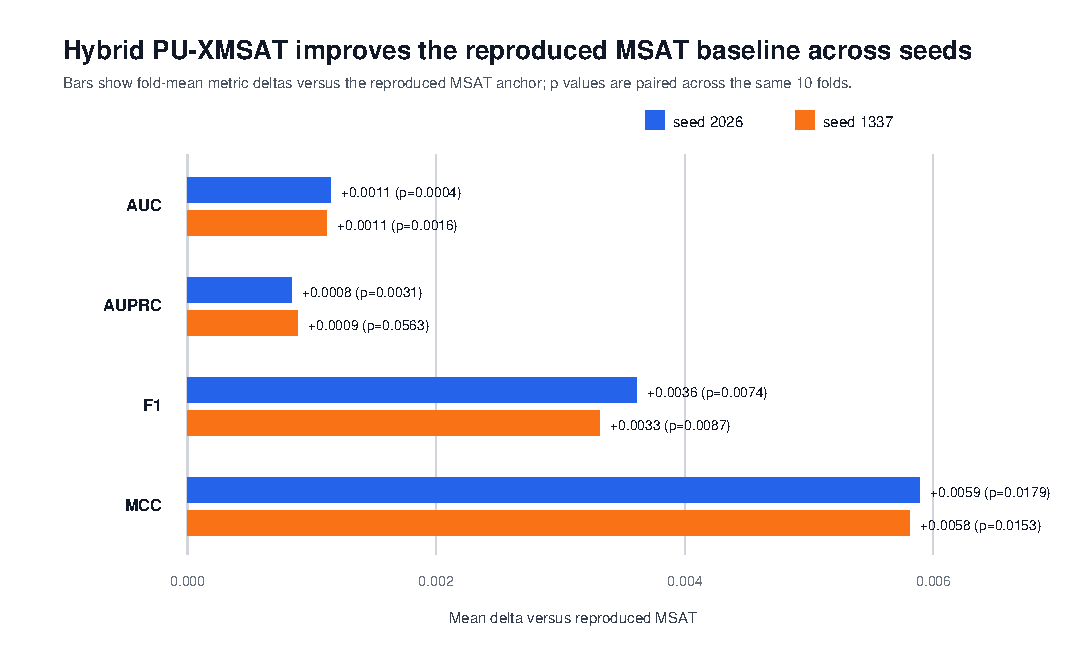
\includegraphics[width=0.82\textwidth]{metric_delta.pdf}
  \caption{Fold-mean metric deltas of hybrid PU-XMSAT versus the reproduced MSAT baseline. The two seed-controlled runs show consistent positive deltas, while AUPRC remains the smallest and most borderline improvement.}
  \Description{Horizontal bar chart with AUC, AUPRC, F1, and MCC on the vertical axis. Blue bars show seed 2026 and orange bars show seed 1337. All deltas are positive, with the largest deltas for MCC and F1.}
  \label{fig:metric-delta}
\end{figure*}

\begin{table}[t]
\caption{Hybrid PU-XMSAT versus the reproduced MSAT baseline.}
\label{tab:baseline-comparison}
\small
\begin{tabularx}{\textwidth}{l l r c r Y}
\toprule
Comparison & Metric & Mean delta & Wins/losses & $p$ value & Interpretation \\
\midrule
Hybrid seed 2026 vs. \msat{} & AUC & +0.001149 & 9/1 & 0.000419 & Significant positive gain \\
Hybrid seed 2026 vs. \msat{} & AUPRC & +0.000834 & 9/1 & 0.003075 & Significant positive gain \\
Hybrid seed 2026 vs. \msat{} & F1 & +0.003613 & 8/2 & 0.007438 & Significant positive gain \\
Hybrid seed 2026 vs. \msat{} & MCC & +0.005889 & 7/3 & 0.017861 & Significant positive gain \\
Hybrid seed 1337 vs. \msat{} & AUC & +0.001121 & 9/1 & 0.001576 & Replicated positive gain \\
Hybrid seed 1337 vs. \msat{} & AUPRC & +0.000888 & 6/4 & 0.056348 & Positive but borderline \\
Hybrid seed 1337 vs. \msat{} & F1 & +0.003316 & 9/1 & 0.008698 & Replicated positive gain \\
Hybrid seed 1337 vs. \msat{} & MCC & +0.005811 & 8/2 & 0.015257 & Replicated positive gain \\
\bottomrule
\end{tabularx}
\end{table}

\subsection{Seed Robustness and Weight Sensitivity}

Across seeds 2026 and 1337, hybrid \px{} was highly stable. The seed range was 0.000028 for AUC, 0.000054 for AUPRC, 0.000297 for F1, and 0.000078 for MCC. A focused weight-sensitivity analysis (Table~\ref{tab:weight-sensitivity}) supported the default unlabeled weight of 0.2 and reliable-negative weight of 0.8 as a balanced setting. Lowering the unlabeled weight to 0.1 weakened all four metrics, while increasing it to 0.4 produced a similar AUC but slightly weaker AUPRC, F1, and MCC.

\begin{table}[t]
\caption{Focused PU weight sensitivity under full-positive hybrid PU-XMSAT with seed 1337. Reliable-negative weight is fixed at 0.8.}
\label{tab:weight-sensitivity}
\small
\begin{tabularx}{\textwidth}{l r r r r Y}
\toprule
Setting & AUC & AUPRC & F1 & MCC & Interpretation \\
\midrule
u0.1/rn0.8 & 0.979932 & 0.977368 & 0.933956 & 0.866775 & Lower unlabeled weight weakens the result \\
u0.2/rn0.8 & 0.980392 & 0.977983 & 0.934767 & 0.868331 & Balanced default \\
u0.4/rn0.8 & 0.980474 & 0.977902 & 0.934410 & 0.867410 & Similar AUC, slightly weaker thresholded metrics \\
\bottomrule
\end{tabularx}
\end{table}

\subsection{Mechanism Subgraph and Contribution Quantification}

We generated a conservative mechanism-interpretation report for selected cases (Table~\ref{tab:contribution}). In the Zhishi--diarrhoea case, the extracted key subgraph contained 11 nodes, 8 edges, and 14 mechanism paths, and all 11 parsed subgraph nodes were quantified. The largest node-level score drop was observed for target 3223 (drop 0.009835), and the largest path-level drop was observed for the compound 523 to target 3223 path (drop 0.010074). In the Fragaria--altered-consciousness case, the key subgraph contained two nodes and one edge, and both parsed nodes were quantified; the largest observed drop was 0.000021. Aggregating the quantified rows yielded 11 positive node perturbation rows and 10 positive path perturbation rows. A split explanation summary further separated 4 component features, 9 target features, and 10 mechanism-path features; the positive entries were 3 component features, 8 target features, and 8 mechanism-path features. The strongest aggregate entries remained target 3223, component 523, and the compound 523--target 3223 path.

\begin{table}[t]
\caption{Mechanism subgraph, local perturbation sensitivity, and aggregate-sensitive entries for selected cases.}
\label{tab:contribution}
\small
\begin{tabularx}{\textwidth}{l Y r r Y}
\toprule
Case & Key subgraph & Top node drop & Top path drop & Interpretation \\
\midrule
Herb 277 to ADR 2931 & 11 nodes, 8 edges, 14 paths & target 3223, 0.009835 & compound 523 to target 3223, 0.010074 & Sensitive path found; external evidence remains direction-conflicting \\
Herb 237 to ADR 3989 & 2 nodes, 1 edge, 1 path & compound 1073, 0.000021 & compound 1073 to target 2586, 0.000021 & Parsed path exists; sensitivity is negligible and evidence unsupported \\
\bottomrule
\end{tabularx}
\end{table}

The aggregate ranking places the strongest positive path sensitivity on \texttt{compound:523;target:3223} and the strongest positive node sensitivity on \texttt{target:3223}, but these ranks are computed from only the two quantified cases and use the local predictor checkpoint. These results support the mechanism workflow shown in Figure~\ref{fig:mechanism-workflow} as triage rather than confirmed biological validation. In particular, negative score drops in the detailed report indicate that masking increased the model score and should not be interpreted as protective biological evidence.

\begin{figure*}[t]
  \centering
  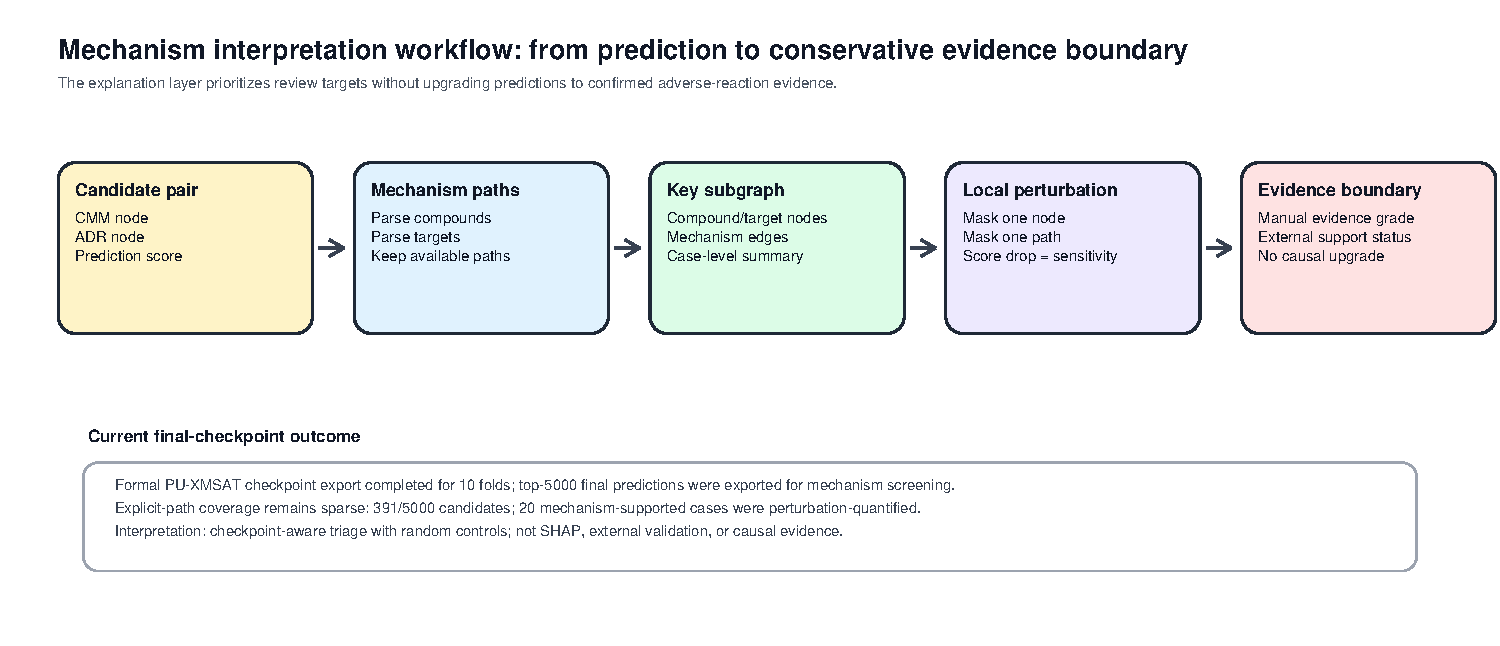
\includegraphics[width=\textwidth]{mechanism_workflow.pdf}
  \caption{Mechanism interpretation and evidence-boundary workflow. The case analysis extracts mechanism paths, assembles a key subgraph, measures local node/path perturbation sensitivity, and then keeps the final claim bounded by manual evidence grading and causal-bias limitations.}
  \Description{A left-to-right workflow from candidate pair to mechanism paths, key subgraph, local perturbation, and evidence boundary. A lower callout summarizes the current Zhishi and Fragaria case-study outcomes.}
  \label{fig:mechanism-workflow}
\end{figure*}

\subsection{Evidence Screening}

The case evidence report contained 16 rows: 15 existing \msat{} Table 5-style candidates and one curated Zhishi--diarrhoea case. Two rows had mechanism/path support and were assigned Grade C, while 14 rows remained prediction-only Grade D candidates. Eight rows had automated literature search records, but no row had manually verified direct literature support. A targeted Direction 3 review queue derived from the perturbation report ranked the Zhishi--diarrhoea pair first by path sensitivity and the Fragaria--altered-consciousness pair second, but both rows remained Grade C boundary cases after manual review and no row was ready for strong-evidence write-up. Therefore, the current evidence workflow should be described as screening and prioritization rather than external validation equivalent to the original Table 5 or Table 6 analyses.

\section{Discussion}

\subsection{Main Findings}

\px{} addresses a methodological limitation exposed during \msat{} reproduction: unobserved CMM--ADR pairs should not automatically be treated as confirmed negatives. By separating observed positives, reliable negatives, and down-weighted unlabeled pairs, \px{} reduces the pressure to learn from potentially mislabeled negative examples. Under the reproduced protocol, the full-positive hybrid setting produced seed-robust gains over \msat{} on AUC, F1, and MCC, with a stable positive but smaller AUPRC trend.

\subsection{Research Value and Practical Use}

The practical value of \px{} is not that it turns graph predictions into confirmed adverse-reaction evidence. Instead, it offers a reproducible way to make CMM safety prediction less dependent on an unrealistic closed-world label assumption. For method developers, the study shows that a reproduced graph model can be improved by changing the supervision construction while leaving the architecture and official folds fixed. For pharmacovigilance researchers, the output is a ranked and mechanism-annotated candidate list that can guide manual review, literature search, and future data collection. For CMM safety studies, the work also clarifies which claims are currently supported: protocol-level prediction improvement and mechanism prioritization are supported, whereas patient-level risk adjustment, external case confirmation, and causal attribution remain future work.

\subsection{Why Hybrid Reliable-Negative Selection Matters}

The hybrid reliable-negative strategy performed better than random sampling in the seed-controlled full-positive setting. This suggests that mechanism-aware reliable-negative scoring contributes useful information for supervision construction. However, this score remains heuristic. It should be interpreted as a practical selection rule rather than proof that selected pairs are true negatives.

\subsection{Interpretability and Evidence Boundaries}

The mechanism layer makes the model output easier to inspect by identifying candidate subgraphs, nodes, paths, and aggregate sensitivity ranks that affect local prediction scores. This is useful for prioritizing cases for manual review and future evidence collection. Nevertheless, local perturbation sensitivity is not equivalent to SHAP attribution, causal effect estimation, or direct biological evidence. The evidence grading results also remain conservative: no current case has been upgraded to direct external support after manual review.

\subsection{Limitations}

This study has several limitations. First, \px{} depends on the quality of the reliable-negative scoring function, which is heuristic and should be validated further. Second, the two-seed robustness analysis supports stability but does not exhaust all sources of stochastic variation. Third, the original \msat{} Table 5 and Table 6 analyses are auxiliary external-validation and interpretation analyses rather than the main performance experiment; the current public-material reproduction does not fully recover these auxiliary claims. Fourth, the current graph data do not include patient-level co-medication, indication, dose, preparation quality, exposure denominators, or reporting propensity. Therefore, the current method should not be interpreted as adjusting for these confounders or estimating causal effects.

\subsection{Threats to Validity}

The main internal-validity threat is that reliable-negative selection is still a heuristic approximation. The hybrid score is useful because it improves the reproduced protocol and remains stable across two seeds, but it does not prove that every selected unobserved pair is a biological non-association. The main construct-validity threat is that the evaluation uses known CMM--ADR labels as the observable target. This target is appropriate for reproducing \msat{} and testing incomplete-label supervision, but it should not be confused with true incidence, clinical severity, or causal risk. The main external-validity threat is that all primary claims are tied to the reproduced \msat{} graph, official folds, and available public materials. Generalization to other CMM resources, ADR vocabularies, or patient-level pharmacovigilance datasets requires a separate study. Finally, the mechanism analysis has a reproducibility boundary: the current local perturbation workflow is sufficient for case triage and hypothesis generation, but a final exported hybrid \px{} checkpoint and a larger manually reviewed case set are needed before making stronger attribution or validation claims.

\subsection{Future Work}

Future work should export an explicit final hybrid \px{} checkpoint for attribution, expand the contribution analysis from selected cases to a larger candidate cohort, and perform targeted external evidence review for high-confidence predictions. If patient-level or pharmacovigilance report-level data become available, causal adjustment strategies could be explored to address co-medication, indication bias, reporting bias, and exposure population differences.

\section{Conclusion}

We presented \px{}, a positive-unlabeled extension of the reproduced \msat{} protocol for CMM adverse reaction prediction. The method improves the supervision assumption by separating observed positives, reliable negatives, and down-weighted unlabeled pairs. Under the reproduced ten-fold protocol, full-positive hybrid \px{} showed seed-robust improvements over the reproduced \msat{} baseline on AUC, F1, and MCC, with a stable positive AUPRC trend. A mechanism-oriented perturbation analysis further supports transparent case triage, while the manuscript maintains conservative boundaries around external validation and causal interpretation.

\section*{Declaration on Generative AI Assistance}

During draft preparation, the authors used AI-assisted tools to support language drafting, result summarization, and manuscript organization. The authors reviewed and edited the content and take responsibility for the accuracy, integrity, and originality of the final manuscript. This statement should be revised to match the final venue policy before submission.

\begin{acks}
TODO: Add funding, institutional support, and supervisor acknowledgements if appropriate.
\end{acks}

\bibliographystyle{ACM-Reference-Format}
\bibliography{references}

\end{document}
